\documentclass[russian]{lecture-notes}

\usepackage[final]{graphicx} % возможность вставлять изображения в текст
\usepackage{subcaption} % пакет нужен, чтобы можно было ставить несколько рисунктов рядом     

\usepackage{amssymb} % для знака пустого множества
\usepackage{amsfonts} % для букв с двойными штрихами (знак натуральных чисел)

\usepackage{tikz}  % для рисования графов
\usetikzlibrary{graphs}

\usepackage{pgfplots}

\usepackage{cancel}
\usepackage{amsmath}

\title{Математическая логика и теория алгоритмов}
\lecturer{Поcов Илья Александрович}
\notesauthor{Блюдин Андрей и Хаматов Вадим}

\begin{document}
	\maketitle

\begin{sloppypar}

\tableofcontents

\section{Математическая логика}

\subsection{Исчисление высказываний}

\subsubsection{Основные понятия}

\begin{definition} 
	Логическая функция ~--- это множество из 2 элементов. Также, логической функцией называют множество логических значений
		
	$B = \{0, 1 \}$, где 0 ~--- это ложь (false), а 1 ~--- это истина (true)
\end{definition}

\begin{definition} 
	Логическая функция от $n$ переменных
	$$f : B^n \rightarrow B$$ 
\end{definition}

\begin{remark}
    Часто логические функции вводят как перечисление возможных аргументов и значений функции при этих аргументах
\end{remark}

\begin{example}
	Введем функцию $f(x,y)$
	
	\begin{table}[h!]
		\centering
		\begin{tabular}{|c|c|c|cl}
			\cline{1-3}
				x & y & f(x,y) & &  \\ \cline{1-3}
				0 & 0 & 0      &  &  \\ \cline{1-3}
				0 & 1 & 1      &  &  \\ \cline{1-3}
				1 & 0 & 1      &  &  \\ \cline{1-3}
				1 & 1 & 1      &  &  \\ \cline{1-3}
		\end{tabular}
		\caption{Таблица истинности для $f(x,y)$}
	\end{table}
	
	Эту же функцию можно задать функцией $f(x,y) = max(x,y)$
\end{example}

\begin{proposition}
    Функция от $n$ переменных может быть $f(x_1, x_2, x_3, \dots, x_n)$
    
    \begin{table}[h!]
  	  	\centering
		\begin{tabular}{|c|c|c|c|l|}
			\hline
			$x_1$ & $x_2$ & ... & $x_n$                   & f($x_1, x_2, \dots, x_n$) \\ \hline
			0    & 0    & ... & 0                      & 0 или 1                  \\ \hline
			...  & ...  & ... & ...                    & 0 или 1                  \\ \hline
			1    & 1    & ... & \multicolumn{1}{l|}{1} & 0 или 1                  \\ \hline
		\end{tabular}
		\caption{Таблица истинности для $f(x_1,x_2, \dots, x_n)$}
	\end{table}
		
	При этом количество всех возможных наборов аргументов равняется $2^n$, а количество всех возможных функций при всех возможных наборах аргументов равняется $2^{2^n}$
\end{proposition}

\begin{corollary}
    Посчитаем количество таких функий для разных $n$
    
    $n = 1 \quad 2^2 = 4$ функций $f(x)$
    
	$n = 2 \quad 2^{2^2} = 16$ функций $f(x,y)$

	$n = 3 \quad 2^{2^3} = 2^8 = 256$ функций $f(x,y,z)$
\end{corollary}

\subsubsection{Функции от 1 переменной (их определения)}

\begin{example}
	Перечислим все возможные функции от 1 переменной
	
	\begin{table}[h!]
	\centering
		\begin{tabular}{|c|c|c|c|l|}
			\hline
			$x$ & $f_1(x)$ & $f_2(x)$ & $f_3(x)$ & $f_4(x)$ \\ \hline
			0 & 0       & 0       & 1       & 1       \\ \hline
			1 & 0       & 1       & 0       & 1       \\ \hline
		\end{tabular}
	\end{table}
	
	Данные функции имеют значение:
	
	$f_1(x) = 0$ ~--- функция 0
	
	$f_2(x) = x$ ~--- функция $x$
	
	$f_3(x) = !x, \bar x, \neg x$, not $x$ ~--- функция отрицания (не $x$)
	
	$f_4(x) = 1$ ~--- функция 1
	
\end{example}

\subsubsection{Функции от 2 переменных (их определения)}

\begin{example}
	Перечислим все возможные функции от 2 переменных
	
	\begin{table}[h!]
	\centering
		\begin{tabular}{|c|c|c|c|c|c|c|c|c|c|}
			\hline
			$x$ & $y$ & $f_1(x)$ & $f_2(x)$ & $f_3(x)$ & $f_4(x)$ & $f_5(x)$ & $f_6(x)$ & $f_7(x)$ & $f_8(x)$ \\ \hline
			0 & 0 & 0       & 0       & 0       & 0       & 0       & 0       & 0       & 0       \\ \hline
			0 & 1 & 0       & 0       & 0       & 0       & 1       & 1       & 1       & 1       \\ \hline
			1 & 0 & 0       & 0       & 1       & 1       & 0       & 0       & 1       & 1       \\ \hline
			1 & 1 & 0       & 1       & 0       & 1       & 0       & 1       & 0       & 1       \\ \hline
		\end{tabular}
		\caption{Таблица истинности для $f(x,y)$}
	\end{table}
	
	Продолжение:
	
	\begin{table}[h!]
	\centering
		\begin{tabular}{|c|c|c|c|c|c|c|c|c|c|}
			\hline
			$x$ & $y$ & $f_9(x)$ & $f_{10}(x)$ & $f_{11}(x)$ & $f_{12}(x)$ & $f_{13}(x)$ & $f_{14}(x)$ & $f_{15}(x)$ & $f_{16}(x)$ \\ \hline
			0 & 0 & 1       & 1       & 1       & 1       & 1       & 1       & 1       & 1       \\ \hline
			0 & 1 & 0       & 0       & 0       & 0       & 1       & 1       & 1       & 1       \\ \hline
			1 & 0 & 0       & 0       & 1       & 1       & 0       & 0       & 1       & 1       \\ \hline
			1 & 1 & 0       & 1       & 0       & 1       & 0       & 1       & 0       & 1       \\ \hline
		\end{tabular}
		\caption{Таблица истинности для $f(x,y)$}
	\end{table}
	
	\textbf{Перечислим основные значения функций:}
	
	$f_2(x,y)$ ~--- это конъюнкция или "лочическое и"  или логическое умножение ($xy, x\&y, x \wedge y$)
	
	$f_7(x,y)$ ~--- это исключающее или ($x+y, x XOR y, x \oplus y$), также данную функцию можно ассоциировать как $(x+y) mod 2$
	
	$f_8(x,y)$ ~--- это логическое или, но ее можно также записать как $max(x,y)$  ($x|y, x \lor y$)
	
	$f_{10}(x,y)$ ~--- это эквивалентность ($x \Leftrightarrow y, x \equiv y, x == y$)
	
	$f_{14}(x,y)$ ~--- это импликация ($x \Rightarrow y, x \rightarrow y$)
	
	Импликация работает так, что истина следует из чего угодно:
	
	лешия не существует $\Rightarrow$ русалок не существует = 1 (1 $\Rightarrow$ 1 = 1)
	
	допса скучная $\Rightarrow$ русалок не существует = 1 (0 $\Rightarrow$ 1 = 1)
	
	русалки существуют $\Rightarrow$ драконы существуют = 1 (0 $\Rightarrow$ 0 = 1)	

	 x $\Rightarrow$ y = 0 только если x = 1, а y = 0

	$f_{12}(x,y)$ ~--- это обратная импликация ($x \Leftarrow y = y \Rightarrow x$)
	
	$f_{9}(x,y)$ ~--- стрелка Пирса ($x \downarrow y = \overline{x \lor y}$)

	$f_{15}(x,y)$ ~--- штрих Шеффера ($x | y = \overline{xy}$)
	
	$f_{3}(x,y)$ ~--- запрет по y ($x > y = \overline{x \Rightarrow y}$)

	$f_{1}(x,y)$ ~--- 0

	$f_{4}(x,y)$ ~--- $x$
	
	$f_{5}(x,y)$ ~--- запрет по x ($x < y = \overline{x \Leftarrow y}$)

	$f_{6}(x,y)$ ~--- $y$
	
	$f_{11}(x,y)$ ~--- не y ($\neg y$)
	
	$f_{13}(x,y)$ ~--- не x ($\neg x$)
	
	$f_{16}(x,y)$ ~--- 1

\end{example}

\begin{definition} 
	Логические выражения ~--- способ задания логических функций с помощью переменных, цифр 0 или 1 и операций:
	
	$\cdot \quad \lor \quad \Rightarrow \quad  \Leftrightarrow \quad + \quad \equiv \quad | \quad \downarrow \quad < \quad >$ 
\end{definition}

\begin{example} 
	Примеры логических выражений:

	$(x \lor y) = $
	
	$(x \Rightarrow yz) \lor (y \equiv z)$
	
	$(0 \Rightarrow x) \lor (1 \Rightarrow y)$
\end{example}

\begin{definition} 
	Значения логического выражения можно записать \textbf{Таблицей истинности}
\end{definition}

\begin{example}
	$f(x, y, z) = (x \lor y)z$
	
	\begin{table}[h!]
		\centering
		\begin{tabular}{|c|c|c|c|}
			\hline
			x & y & z & f(x,y,z) \\ \hline
			0 & 0 & 0 & 0        \\ \hline
			0 & 0 & 1 & 0        \\ \hline
			0 & 1 & 0 & 0        \\ \hline
			0 & 1 & 1 & 1        \\ \hline
			1 & 0 & 0 & 0        \\ \hline
			1 & 0 & 1 & 1        \\ \hline
			1 & 1 & 0 & 0        \\ \hline
			1 & 1 & 1 & 1        \\ \hline
		\end{tabular}
	\end{table}
\end{example}

\begin{remark}
	Порядок строчек в таблеце истинности может быть любым, но лучше использовать как у двоичных чисел    
\end{remark}

\begin{proposition}
    Таблицы истинности часто считают постепенно
	
	\begin{table}[h!]
		\centering		
		\begin{tabular}{|c|c|c|c|l|}
			\hline
			x & y & z & $x \lor y$ & $(x \lor y)z$  \\ \hline
			$\dots$ & $\dots$ & $\dots$ & $\dots$ & $\dots$ \\ \hline
			$\dots$ & $\dots$ & $\dots$ & $\dots$ & $\dots$ \\ \hline
		\end{tabular}
	\end{table}
\end{proposition}

\subsubsection{Приоритеты операций}
	
	$$\neg$$
	
	$$\cdot$$
	
	$$\lor$$
	
	$$+ \quad \equiv$$
	
	$$\Rightarrow \quad \Leftarrow$$
	
	$$| \quad \downarrow \quad < \quad >$$
	
\begin{example}
	Примеры приоритетов операций:
	
	$\neg x \lor y = (\neg x) \lor y$
	
	$x \lor y z = x \lor (y z)$
	
	$x \Rightarrow y \lor z = x \Rightarrow (y \lor z)$
\end{example}	

\subsubsection{Алгебраические преобразования логических выражений}

\begin{definition} 
	Алгебраические преобразования логических выражений ~--- изменяем выражения по правилам, обычно в сторону упрощения
\end{definition}

\begin{example}
	$(0 \Rightarrow x) \lor (1 \Rightarrow y) = 1 \lor (1 \Rightarrow y) = 1$
\end{example}

\begin{proposition*}
    $$\overline{\overline{x}} = x$$
    
    \textbf{Доказательство:}
    
    \begin{table}[h!]
		\centering		
		\begin{tabular}{|c|c|c|}
			\hline
			$x$ & $\overline{x}$ & $\overline{\overline{x}}$ \\ \hline
			0 & 1 & 0 \\ \hline
			1 & 0 & 1 \\ \hline
		\end{tabular}
	\end{table}

\end{proposition*}

\begin{proposition*}
    При $\lor$:
    
    $$1 \lor x = 1$$
    
    $$0 \lor x = x$$
    
    $$x \lor y = y \lor x$$
\end{proposition*}

\subsubsection{Таблица эквивалентных логических выражений}

\begin{proposition}
    $x \lor y = y \lor x $ - симметричность
    

    $x \lor 0 = x$
    

    $x \lor 1 = 1$
    

    $x \lor x = x$
    

    $x \lor \overline{x} = 1 $
        
        
        $\qquad$ \textbf{Доказательство:}
        
        
    \begin{table}[h!]
		\centering		
		\begin{tabular}{|c|c|c|}
			\hline
			$x$ & $\overline{x}$ & $x \lor \overline{x}$ \\ \hline
			0 & 1 & $0 \lor 1 = 1$ \\ \hline
			1 & 0 & $1 \lor 0 = 1$ \\ \hline
		\end{tabular}
	\end{table}
        
    $xy = yx $

    $x*0 = 0$
    
    $x*1 = x$

    $x*x = x$

    $x* \overline{x} = 0$

    $x+y = y + x$
    
    $x + 0 = x$

    $x + 1 = \overline{x}$

    $x + x = 0$

    $x + \overline{x} = 1 $

\end{proposition}

\begin{proposition}
    
    $x \lor (y\lor z) = (x \lor y ) \lor z$ - ассоциативность
    
    Ассоциативность означает,что порядок скобок не важен 
    
    \begin{example} $x \Rightarrow y \neq y \Rightarrow x$ - не симметричная функция
    
    $$$$
    
        \textbf{Доказательство: }
        
    \begin{table}[h!]
        \centering	
        \begin{tabular}{|l|l|l|}
            \hline
            x y & $x \Rightarrow y$ & $y \Rightarrow x$ \\ \hline
            0 0 & 1 & 1 \\ \hline
            0 1 & 1 & 0 \\ \hline
            1 0 & 0 & 1 \\ \hline
            1 1 & 1 & 1 \\ \hline
        \end{tabular}
    \end{table}
    
    \end{example}
    
    \begin{remark}
        $x \Rightarrow y \neq y\Rightarrow x$
    \end{remark}
        
$x \Rightarrow 0 = \overline{x}$

$0 \Rightarrow x = 1$
 $$$$

\textbf{Доказательство: }

\begin{table}[h!]
\centering
\begin{tabular}{|l|l|}
\hline
x & $x \Rightarrow 0$ \\ \hline
0 & $0 \Rightarrow 0 = 1$ \\ \hline
1 & $1 \Rightarrow 0 = 0$ \\ \hline
\end{tabular}
\end{table}

$x\Rightarrow 1 = 1$

$1 \Rightarrow x = x$

$x \Rightarrow x = 1$

$x \Rightarrow \overline{x} = \overline{x}$

$\overline{x} \Rightarrow x = x$

$\overline{x} \Rightarrow y \Rightarrow z$ договоримся, что это $x \Rightarrow y (y\Rightarrow z) \neq (x \Rightarrow y) \Rightarrow z$

\begin{table}[h!]
\centering
\begin{tabular}{|l|l|l|l|l|}
\hline
x y z  & $x \Rightarrow y$ & $y \Rightarrow z$ & $x \Rightarrow (y \Rightarrow z)$ & $(x \Rightarrow y) \Rightarrow z$ \\ \hline
0 0  0 & 1               & 1                 & 1                                 & 0                                 \\ \hline
0 0 1  & 1               & 1                 & 1                                 & 1                                 \\ \hline
0 1 0  & 1               & 0                 & 1                                 & 0                                 \\ \hline
0 1 1  & 1               & 1                 & 1                                 & 1                                 \\ \hline
1 0 0  & 0               & 1                 & 1                                 & 1                                 \\ \hline
1 0 1  & 0               & 1                 & 1                                 & 1                                 \\ \hline
1 1 0  & 1               & 0                 & 0                                 & 0                                 \\ \hline
1 1 1  & 1               & 1                 & 1                                 & 1                                 \\ \hline
\end{tabular}
\end{table}

$x \Leftrightarrow y = y \Leftrightarrow x$

$x \Leftrightarrow 0 = \overline{x}$

$x \Leftrightarrow 1 = x$

$x \Leftrightarrow x =1$

$x \Leftrightarrow \overline{x} = 0$

$x \Leftrightarrow (y\Leftrightarrow z) = (x \Leftrightarrow y) \Leftrightarrow z$ - ассоциативно

\end{proposition}

\begin{proposition}

Дистрибутивность

$(x \lor y) z = xz \lor yz$

$(x+y)z = xz + yz$ по таблице истинности

$(x \& y ) \lor z$ ($xy \lor z = (x \lor z)(y \lor z)$

$(x \lor y) \& z = (x \& z) \lor (y \& z)$

$(x \& y) \lor z = (x \lor z) \& (y\lor z)$

\begin{remark}

$ $
    $(x_{1} \lor x_{2} \lor x_{3}) (y_{1} \lor y_{2}) = (x_{1} \lor x_{2} \lor x_{3})y_{1} \lor (x_{1} \lor x_{2} \lor x_{3})y_{2} = x_{1}y_{1} \lor x_{2}y_{1} \lor x_{3}y_{1} \lor x_{1}y_{2} \lor x_{2}y_{2} \lor x_{3}y_{2}$

    $xy \lor z = (x \lor z)(y\lor z) = xy \lor xz \lor zy \lor zz = xy \lor  xz \lor zy \lor z = xy \lor xz \lor zy \lor z*1 = xy \lor z(x\lor y \lor 1) = xy \lor z$ сошлось
    
\end{remark}

$x+y = \overline{x\Rightarrow}y$ - смотри Таблицу истинности

$(x\Rightarrow y)(y\Rightarrow x) = x \Rightarrow y$

\subsubsection{Многочлены Жегалкина}

    \begin{remark}
    
        Одну и ту же функцию можно записать по разному.
    
    \end{remark}
    
    В алгебре: $f(x) = 1 +x = x + 1 = x + 5 - 4 = sin(x-x) + x = ...$
    
    В логике: $f(x,y) = x \lor y = x \lor y \lor 0 = (x \lor y)(\overline{y} \lor y = x\overline{y} \lor y$ (= - дистрибутивность)
    
    \textbf{Многочлены Жегалкина для логической формулы}
    
    
    \begin{definition}
        $f(x_{1}......x_{n}$) - это многочлен с переменными xi, конспектами 0,1 и со степенями переменных $\leqslant$ 1. Это многочлены от xi $\mathbf{Z_{2}}$
    \end{definition}
    
    \begin{example}
    
        $f(x,y,z) = 1 + x + yz + xyz$
        
        $1 + x \qquad \qquad xy+xyz$
        
        $1 + xy$
    \end{example}
    
    Не многочлены
    
    $1 + x + (y \lor z)$
    
    $1 + x + z^{2}$ нельзя степень 2
    
    
    \begin{remark}
        В общем случае многочлен от 1 переменной ($a_{i} =$ 0 или 1)
        
        $a_{0} + a_{1}x$
        
        от 2ух: $a_{0} + a_{1}x+a{2}y+a{3}xy$
        
        от 3ех: $a_{0} + a_{1}x + a_{2}y + a_{3}z + a_{4}xy + a_{5}xz + a_{6}yz + a_{7}xyz$
        
        \end{remark}
        
        В общем случае $f(x1....x_{n}$) $a_{0} + a_{1}x_{1} + ... + a_{n}x_{n} + ax_{1}x_{2} + ax_{1}x_{3}$ + ... (все пары переменных) + $ ax_{1}x_{2}x_{3}+ax_{1}x_{3}x_{2} \leftarrow $все тройки перменных$ + ax_{1}x_{2}x_{3}...x_{n}$
        
        \begin{definition}
            $\forall f(x_{1}...x_{n})$ - логические функция $\exists!$ многочлен Жегалкина $g(x_{1}...x_{n}) : f = g$
        \end{definition}
        
        \begin{remark}
            Всего 4 функции от 1ой переменной
            
            $f(x) = 0 = \overline{x} = 0 + 0x$
            
            $f(x) = 1 = 1 = 1 + 0x$
            
            $f(x) = x = x = 0 + 1x$
            
           $f(x) = \overline{x} = 1 + x = 1 + 1x$
        \end{remark}
    
    \textbf{Докозательство:}
    
        \begin{definition}
            Разные многочлены - это разные логические функции т.е. $f(x_{1} ... x_{n} = a_{0} + ... + a_{1}x_{1} ... x_{n}$
            
            $g(x_{1}...x_{n}) = b_{0} + ... + bx_{1} ... x_{n}$
            
            $\exists!$ : $a_{i} \neq b_{i}$ различающийся
            
        \end{definition}
        
        \qquad \textbf{Доказательство:}
        
        Возьмем индекс с самым большик количеством переменных
        
        $f(x,y,z) = 1 + x + xy + xyz = ... + 1x + Dy + Dz + 1xy$
        
        $g(x,y,z) = 1 + y + z + xyz ... + Dx + 1y + 1z$
        
        для переменных этого слагаемого подставим 1 0xy 
        
        для остальных переменных : 0
        
        [ В примере $x=1,y=0,z=0 : f(1,0,0)$ и $g(1,0,0)$ ]
        
        и в f и в g все другие слагаемые равны 0
        
            Теперь f(...) и g(...) 
            
                $f(...) = a_{i}x{1}x_{2}x_{3} \neq b_{i}x_{1}x_{2}x_{3}$ $\Rightarrow f(x_{1}...x_{n}$) $\neq y$ 
                
    \qquad \textbf{Доказательство:}
    
    Проверим, что многочленов Жегалкина столько, сколько функций:
    
        Посчитаем
        
        $a_{0} + a_{1}x_{1}+ ... + a_{1}x_{1}x_{2}...x_{n}$
        
        Сколько слагаемых:
        
        1) 1 слагаемых без переменных
        
        n слагаемых с переменной
        
        \qquad $a_{1}x_{1} + ... + a_{n}x_{n}$
        
        $C_{n}^{2}$ - слагаемых с 2 - мя переменными
        
        $C_{n}^{3}$ - слагаемых с 3 - мя переменными
        
        $C_{n}^{n}$ - слагаемых с n переменными
        
        Всего : $ C_{n}^{0} + C_{n}^{1} + C_{n}^{2} + ... C_{n}^{n} = 2^{n}((1+1)^{2}) $
        
    \begin{example}
            
    $a_{0} + a_{1}x$ - 2 слагаемых
            
    $a_{0} + a_{1}x + a_{2}y+a_{3}xy - 2^2 = 4$ слагаемых
    
    2) Все слагаемых имею вид: $x_{1},x_{2},x_{3}...x_{n}$ (0 или 1) - $2^n$ слагаемых
    
    Итого: многочлен Жегалкина от n переменных 
    \end{example}
    
    
    \begin{problem}
    Сколько разных многочленов?
    
    Это столько же, сколько логический функций
    
    Итог: 
    
    \textbf{Следствие:} Любая логическая функция может быть представлена в виде многочлена Жегалкина
    
    \end{problem}
    
    \begin{example}
    
        $f(x,y) = x \lor y$
        
        $f(x,y) = x*y$ - уже многочлен Жегалкина
        
        \textbf{Метод неопределенных коэффициентов:}
        
        
        Подберем $x \lor y = a_{0} + a_{1}x + a_{2}y + a_{3}xy$
        
        $f(0,0) = 0$
        
        $f(0,0) = a_{0} + a_{1}*0 + a_{2}*0 + a_{3}...$
        
        $f(1,0) = 1 \lor 0 = 1$
        
        $f(1,0) = a_{0} + a_{1} = a_{1}$ ($a_{0} = 0, \Rightarrow a_{1} = 1$
        
        $f(0,1) =$ аналогично $\Rightarrow a_{1} = 1$
        
        $f(x,y) = x+y + a_{3}xy$
        
        $f(1,1) = 1 \lor 1 = 1$
        
        $f(1,1) = 1 + 1 + a_{3} = 0 + a_{3} = a_{3}$, $a_{3}=1$
        
        Ответ: $x\lor y = x+y+xy$
        
    \end{example}

\end{proposition}

\textbf{Многочлены Жегалкина от 1 переменной:}

\begin{table}[h!]
	\centering
	\begin{tabular}{|c|c|}
		\hline
		$f(x)$ & Мн Ж  \\ \hline
		0    		   & 0     \\ \hline
		1    		   & 1     \\ \hline
		$x$          & $x$     \\ \hline
		$\bar{x}$ & $1 + x$ \\ \hline
	\end{tabular}
\end{table}

\textbf{Многочлены Жегалкина от 2 переменных:}

\begin{table}[h!]
	\centering
	\begin{tabular}{|c|c|}
		\hline
		$f(x)$ & Мн Ж  \\ \hline
		0    		   & 0     \\ \hline
		1    		   & 1     \\ \hline
		$xy$          & $xy$     \\ \hline
		$x + y$ & $x + y$ \\ \hline
		$x \lor y$ & $x + y + xy$ \\ \hline
	\end{tabular}
\end{table}

\textbf{Формулы:}

\begin{enumerate}
	\item 	$\overline{xy} = \neg (xy) = \overline{x} \lor \overline{y} $
	\item $\overline{x \lor y} = \neg (x \lor y) = \overline{x} \cdot \overline{y} = \overline{x} \: \overline{y}$
\end{enumerate}

\begin{remark}
	$\overline{xy} \neq \overline{x} \cdot \overline{y} = \overline{x} \: \overline{y}$
\end{remark}

\textbf{Докозательство формул через таблицу истинности:}

\begin{table}[h!]
	\centering	
	\begin{tabular}{|c|c|c|c|}
		\hline
		$x$ & $y$ & $\overline{x \lor y}$ & $\overline{x} \cdot \overline{y}$ \\ \hline
		0 & 0 & 1   & 1   \\ \hline
		0 & 1 & 0   & 0   \\ \hline
		1 & 0 & 0   & 0   \\ \hline
		1 & 1 & 0   & 0   \\ \hline
\end{tabular}
\end{table}

\subsubsection{Получение многочлена Жегалкина через алгебраические упрощения}

\begin{enumerate}
	\item{
		\textbf{Многочлен Жегалкина для $\lor$}

		$x \lor y = (x = \overline{a}, y = \overline{y}) = \overline{ab} = \overline{\overline{x} \cdot \overline{y}} = \overline{(1 + x)(1 + y)} = 1 + (1 + x)(1 + y) = 1 + 1 + x + y + xy = \underline{x + y + xy}$
	} 

	\item{
		\textbf{Многочлен Жегалкина для $\Leftrightarrow$}

		$x \Leftrightarrow y = \overline{x + y} = \underline{1 + x + y}$
	}

	\item{
		\textbf{Многочлен Жегалкина для $\Rightarrow$}	
		
		$x \Rightarrow y = \overline{x} \lor y = (1 + x) \lor y = (1 + x) + y + (1 + x)y = 1 + x + y + y + xy = \underline{1 + x + xy}$ 
	}
\end{enumerate}

\begin{remark}

	Если есть логическая формула, то ее можно приветси к форме многочлена Жегалкина двумя способами:

\begin{enumerate}
	\item{
		метод неопределенных коэффициентов:
		
		$a_0 + a_1x + a_2y + a_3z + \dots + axyz$	
	}
	\item{
		метод алгебраических преобразований	
	}
\end{enumerate}	

\begin{example}
	$x \lor y = \overline{\overline{x} \cdot \overline{y}} = \dots = x + y + xy$
\end{example}

\begin{example}
	$x \Rightarrow y = \overline{x} \lor y = \dots = 1 + x + xy$
\end{example}

\begin{example}
	$x \Rightarrow (y \lor \overline{z}) = x \Rightarrow (y + \overline{z} + y \cdot \overline{z}) = x \Rightarrow (y + (1 + z) + y \cdot (1 + z))  = x \Rightarrow (y + 1 + z + y + yz) = x \Rightarrow (1 + z + yz) = 1 + x + x(1 + z + yz) = 1 + x + x + xz + xyz = 1 + xz + xyz $
\end{example}

\end{remark}

\textbf{Поймем, что:}
	$(x \Leftrightarrow y) \Leftrightarrow z = x \Leftrightarrow (y \Leftrightarrow z)$
	
	$x \Leftrightarrow y \Leftrightarrow z = (1 + x + y) \Leftrightarrow z = 1 + (1 + x + y) + z  = 1 + 1 + x + y + z = x + y + z $
	
\textbf{Вывод:}

	Заранее не ясно, сложно ли привести логическую формулу к многочлену Жегалкина	

\subsubsection{Дизъюнктивно-нормальная форма (ДНФ)}

\begin{definition} 
	Литерал ~--- это переменная или отрицание переменной
\end{definition}

\begin{example}
	$x, \overline{x}, y, \overline{y}, z, \overline{z}$
\end{example}

\begin{definition} 
	Конъюнктор ~--- конъюнкция литералов
\end{definition}

\begin{example}
	$x\overline{y}, xyz, \overline{x} \: \overline{y} \: \overline{z}, \overline{x}z,$ ноль (пустой конъюнкт).
\end{example}

\begin{definition} 
	Логическое выражение имеет ДНФ, если она является дизъюнкцией конъюнкторов
\end{definition}

\begin{example}
	$x\overline{y} \lor \overline{x} \: \overline{z} \lor z \lor \overline{x} \: \overline{y}$ ~--- ДНФ
\end{example}

\begin{example}
	$xy \lor \overline{x} \: \overline{y}$ ~--- ДНФ
\end{example}

\begin{example}
	$x \lor y$ ~--- ДНФ
\end{example}

\begin{example}
	$xy$ ~--- ДНФ
\end{example}

\begin{example}
	не ДНФ ~--- $\overline{xy} = \overline{x} \lor \overline{y}$ ~---  ДНФ
\end{example}

\begin{example}
	не ДНФ ~--- $x \Rightarrow yz = \overline{x} \lor yz$ ~---  ДНФ
\end{example}

\textbf{Построение ДНФ по таблице истинности функции:}

	алгоритм на примере трех переменных

\begin{table}[h!]
	\centering
	\begin{tabular}{|c|c|c|c|c|}
		\hline
		$x$ & $y$ & $z$ & $f(x, y ,z)$ &     \\ \hline
		0 & 0 & 0 & 0 &     \\ \hline
		0 & 0 & 1 & 0 &     \\ \hline
		0 & 1 & 0 & 1 & $\overline{x} \: y \: \overline{z}$ \\ \hline
		0 & 1 & 1 & 1 & $\overline{x} \: yz$ \\ \hline
		1 & 0 & 0 & 0 &     \\ \hline
		1 & 0 & 1 & 0 &     \\ \hline
		1 & 1 & 0 & 1 & $xy \: \overline{z}$ \\ \hline
		1 & 1 & 1 & 0 &     \\ \hline
	\end{tabular}
\end{table}

	Берем строки из столбца $f(x, y, z)$, где значения в столбце равны 1
	
	Допустим есть строка: $x = a_1, y = a_2, z = a_3$ ($a$ могут быть как 0, так и 1)
	
	В ответ добавляется конъюнкт $xyz$ (0 $\Rightarrow$ отрицание, 1 $\Rightarrow$ не отрицание)
	
	Ответ: $f(x, y, z) = \overline{x} \: y \: \overline{z} \lor \overline{x} \: yz \lor xy \: \overline{z}$

\textbf{Докозательство корректности алгоритма:}

Когда полученный ДНФ = 1?

Когда есть конъюнкт равный 1

\begin{enumerate}
	\item{
		Если первый конъюнкт равняется 1 (в примере 	$\overline{x} \: y \: \overline{z}  = 1)$ 

		$\Rightarrow $ все литералы конъюнкта равняются 1

		$\Rightarrow$ в примере $\overline{x} = 1 \quad y = 1 \quad \overline{z} = 1$

		$ \qquad \qquad \qquad x = 0 \quad y = 1 \quad z = 0$	
	}
	\item{
		Если второй конъюнкт равняется 1
		
		$\Rightarrow$ в примере $x = 0 \quad y = 1 \quad z = 1$ ~--- строка из таблицы истинности	
	}
	\item{
		То же самое с третьим конъюнктом
	}
\end{enumerate}

Посмотрим таблицу с этими конъюнктами:

\begin{table}[h!]
	\centering
	\begin{tabular}{|c|c|c|c|c|c|c|}
		\hline
		$x$ & $y$ & $z$ & $\overline{x} \: y \: \overline{z}$ & $\overline{x} \: yz$ & $xy \: \overline{z}$ & $f(x, y, z)$ \\ \hline
		0 & 0 & 0 & 0   & 0   & 0   & 0 \\ \hline
		0 & 0 & 1 & 0   & 0   & 0   & 0 \\ \hline
		0 & 1 & 0 & 1   & 0   & 0   & 1 \\ \hline
		0 & 1 & 1 & 0   & 1   & 0   & 1 \\ \hline
		1 & 0 & 0 & 0   & 0   & 0   & 0 \\ \hline
		1 & 0 & 1 & 0   & 0   & 0   & 0 \\ \hline
		1 & 1 & 0 & 0   & 0   & 1   & 1 \\ \hline
		1 & 1 & 1 & 0   & 0   & 0   & 0 \\ \hline
	\end{tabular}
\end{table}

\begin{remark}
	У одной функции могут быть разные ДНФ
\end{remark}

\begin{example}
	$\underline{\overline{x} \: y \: \overline{z} \lor \overline{x} \: yz \lor xy \: \overline{z}} = \overline{x} \: y (\overline{z} \lor z) \lor xy \: \overline{z} = \underline{\overline{x} \: y \lor xy \: \overline{z}}$ ~--- подчеркнутые выражения являются ДНФ
\end{example}

\begin{example}
	$\underline{\overline{x} \: y \: \overline{z} \lor \overline{x} \: yz \lor xy \: \overline{z}} = \overline{z} \: y (\overline{x} \lor x) \lor zy \: \overline{x} = \underline{\overline{z} \: y \lor zy \: \overline{x}} = \underline{y \: \overline{z} \lor \overline{x} \: yz \lor \overline{x} \: x \lor z \: \overline{z}}$ ~--- подчеркнутые выражения являются ДНФ
\end{example}

Получить ДНФ для логической функции/формулы можно:
\begin{enumerate}
	\item по таблице истинности
	\item с помощью алгебраических преобразований
\end{enumerate}

\begin{example}
	\begin{enumerate}
		\item $\overline{x} = \overline{x}$
		\item $x \lor y = x \lor y$
		\item $x \cdot y = x \cdot y$
		\item $x \Rightarrow y = \overline{x} \lor y$
		\item $x \Leftrightarrow y = (x \Rightarrow y)(y \Rightarrow x) = (\overline{x} \lor y)(\overline{y} \lor x) = \overline{x} \: \overline{y} \lor \overline{x} \: x \lor y \: \overline{y} \lor yx = \overline{x} \: \overline{y} \lor xy $
		
		\begin{table}[h!]
			\centering
			\begin{tabular}{|c|c|c|}
				\hline
				$x$ & $y$ & $x \Leftrightarrow y$ \\ \hline
				0 & 0 & 1  \\ \hline
				0 & 1 & 0  \\ \hline
				1 & 0 & 0  \\ \hline
				1 & 1 & 1  \\ \hline
			\end{tabular}
		\end{table}
		
		\item{ $x + y = \overline{x \Leftrightarrow y} = \overline{\overline{x} \: \overline{y} \lor xy} \dots$
		
			$ = \overline{\overline{x} \: y} \lor \overline{x \lor \overline{y}} = \overline{\overline{x}} \cdot \overline{y} \lor \overline{x} \cdot \overline{\overline{y}} = x \: \overline{y} \lor \overline{x} \: y$
		}
		\item $x \Rightarrow (y + z) = \overline{x} \lor (y + z) = \overline{x} \lor \overline{y} \: z \lor y \: \overline{z}$
	\end{enumerate}
\end{example}

\subsubsection{Задача (не) выполнимости}

Дана логическая формала в ДНФ

	Проверить, бывает ли она равна 0?

$\overline{x} \: \overline{y} \lor x \lor y  ?= 0$

$x = 0, y = 0 \Rightarrow \overline{x} \: \overline{y} = 1$

$\Rightarrow$ данный ДНФ не может быть равным 0

	Эта задача обладает особенностью:

\begin{enumerate}
	\item если знать значения переменных (ответ), то их легко можно быстро проверить
	\item подобрать значения переменных для 0 ~--- нет
\end{enumerate}

	Нет известного алгоритма, который "принципиально" быстрее полного перебора

У этой задачи класс NP выполнимости (ответ легко проверить, а найти его простым способом невозможно)

\begin{corollary}
	То к чему сводится задача (не) выполнимости тоже сложна
	\begin{enumerate}
		\item упростить логическое выражение
		\item поиск минимального ДНФ
	\end{enumerate}
\end{corollary}

\subsubsection{Запись таблиц истинности в виде графика}

	Формула  = $f(x, y, z) = x + y$

	$$f(0, 0) = 0$$
	
	$$f(0, 1) = 1$$
	
	$$f(1, 0) = 1$$
	
	$$f(1, 1) = 0$$

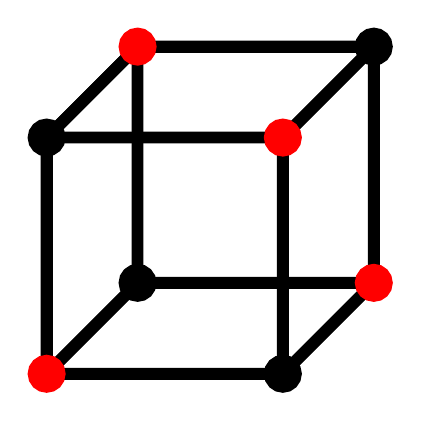
\begin{tikzpicture}[scale=3,line width=1.5mm]

\draw [circle] (1,0,0) -- (1,0,1) -- (1,1,1) -- (1,1,0) -- cycle;
\draw [circle] (0,0,0) -- (0,0,1) -- (0,1,1) -- (0,1,0) -- cycle;

\draw [circle] (0,0,0)   -- (1,0,0)  -- (1,0,1)  -- (0,0,1)  -- cycle;
\draw [circle] (0,1,0)   -- (1,1,0)  -- (1,1,1)  -- (0,1,1)  -- cycle;

\draw [circle] (0,0,0)  node[draw, fill = black] (nodeA) {}  -- (1,0,0)  node[draw, fill = red, red] (nodeA) {}  -- (1,1,0)  node[draw, fill = black] (nodeA) {}  -- (0,1,0)  node[draw, fill = red, red] (nodeA) {}  -- cycle;
\draw [circle] (0,0,1)  node[draw, fill = red, red] (nodeA) {}  -- (1,0,1)  node[draw, fill = black] (nodeA) {}  -- (1,1,1)  node[draw, fill = red, red] (nodeA) {}  -- (0,1,1)  node[draw, fill = black] (nodeA) {}  -- cycle;

\end{tikzpicture}


\subsubsection{Задача минимизации ДНФ}

	Данная задача тоже является сложной, также как и задача (не) выполнимости
	
	Дана логическая функция (в виде ДНФ). Необходимо найти самую короткую ДНФ эквивалентную данной.
	
	Минимальной ДНФ считается та, где меньше количество литералов и дизъюнкций
	
\begin{example}
	$\overline{x} \: \overline{y} \lor z$ короче, чем $xy \lor yz$
\end{example}

\begin{remark}
	Далее рассматриваться все будет для функции от 3 переменных $f(x, y, z)$
\end{remark}

\begin{remark}
	Какова таблица истинности $xyz = abc$, где $a = 0$ или $1, b = 0$ и $1, c = 0$ или $1$
	
	$0 \Rightarrow$ надо поставить отрицание
	
	$1 \Rightarrow$ нет отрицания
\end{remark}

\begin{example}
	$f(x, y, z) = \overline{x} \: y \: \overline{z}$
	
	Если $\overline{x} \: y \: \overline{z} = 1$
	
	$\Rightarrow \overline{x} = 1,  y = 1, \overline{z} = 1$ 
	
	$\Rightarrow x = 0,  y = 1, z = 0$

	$\Rightarrow x = a, y = b, z = c$

	$\Rightarrow a = 0, b = 1, c = 0$

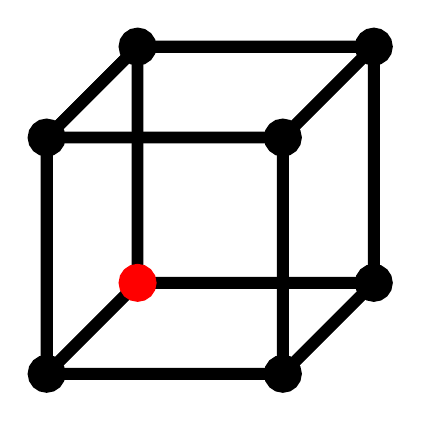
\begin{tikzpicture}[scale=3,line width=1.5mm]

\draw [circle] (1,0,0) -- (1,0,1) -- (1,1,1) -- (1,1,0) -- cycle;
\draw [circle] (0,0,0) -- (0,0,1) -- (0,1,1) -- (0,1,0) -- cycle;

\draw [circle] (0,0,0)   -- (1,0,0)  -- (1,0,1)  -- (0,0,1)  -- cycle;
\draw [circle] (0,1,0)   -- (1,1,0)  -- (1,1,1)  -- (0,1,1)  -- cycle;

\draw [circle] (0,0,0)  node[draw, fill = red, red] (nodeA) {}  -- (1,0,0)  node[draw, fill = black] (nodeA) {}  -- (1,1,0)  node[draw, fill = black] (nodeA) {}  -- (0,1,0)  node[draw, fill = black] (nodeA) {}  -- cycle;
\draw [circle] (0,0,1)  node[draw, fill = black] (nodeA) {}  -- (1,0,1)  node[draw, fill = black] (nodeA) {}  -- (1,1,1)  node[draw, fill = black] (nodeA) {}  -- (0,1,1)  node[draw, fill = black] (nodeA) {}  -- cycle;

\end{tikzpicture} 
 
\end{example}



\begin{example}
	$f(x, y, z) = xy$
	
	Если $xy = 1$
	
	$\Rightarrow x = 1,  y = 1$

	$\Rightarrow x = a, y = b$

	$\Rightarrow a = 1, b = 1$
	 
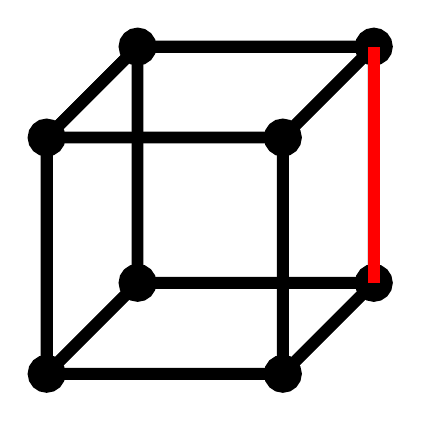
\begin{tikzpicture}[scale=3,line width=1.5mm]

\draw [circle] (1,0,0) -- (1,0,1) -- (1,1,1) -- (1,1,0) -- cycle;
\draw [circle] (0,0,0) -- (0,0,1) -- (0,1,1) -- (0,1,0) -- cycle;

\draw [circle] (0,0,0)   -- (1,0,0)  -- (1,0,1)  -- (0,0,1)  -- cycle;
\draw [circle] (0,1,0)   -- (1,1,0)  -- (1,1,1)  -- (0,1,1)  -- cycle;

\draw [circle] (0,0,0)  node[draw, fill = black] (nodeA) {}  -- (1,0,0)  node[draw, fill = black] (nodeA) {}  -- (1,1,0)  node[draw, fill = black] (nodeA) {}  -- (0,1,0)  node[draw, fill = black] (nodeA) {}  -- cycle;
\draw [circle] (0,0,1)  node[draw, fill = black] (nodeA) {}  -- (1,0,1)  node[draw, fill = black] (nodeA) {}  -- (1,1,1)  node[draw, fill = black] (nodeA) {}  -- (0,1,1)  node[draw, fill = black] (nodeA) {}  -- cycle;

\draw [red] (1,0,0) -- (1,1,0);

\end{tikzpicture} 

	Аналогично, $f(x, y, z) = \overline{y} \: \overline{z}$
	
	ребро: $y = 0, z = 0, x = ?$ ~--- не важно 

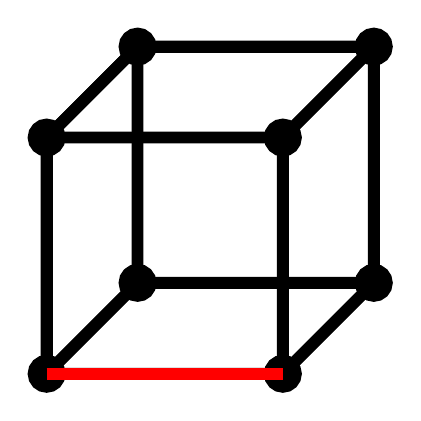
\begin{tikzpicture}[scale=3,line width=1.5mm]

\draw [circle] (1,0,0) -- (1,0,1) -- (1,1,1) -- (1,1,0) -- cycle;
\draw [circle] (0,0,0) -- (0,0,1) -- (0,1,1) -- (0,1,0) -- cycle;

\draw [circle] (0,0,0)   -- (1,0,0)  -- (1,0,1)  -- (0,0,1)  -- cycle;
\draw [circle] (0,1,0)   -- (1,1,0)  -- (1,1,1)  -- (0,1,1)  -- cycle;

\draw [circle] (0,0,0)  node[draw, fill = black] (nodeA) {}  -- (1,0,0)  node[draw, fill = black] (nodeA) {}  -- (1,1,0)  node[draw, fill = black] (nodeA) {}  -- (0,1,0)  node[draw, fill = black] (nodeA) {}  -- cycle;
\draw [circle] (0,0,1)  node[draw, fill = black] (nodeA) {}  -- (1,0,1)  node[draw, fill = black] (nodeA) {}  -- (1,1,1)  node[draw, fill = black] (nodeA) {}  -- (0,1,1)  node[draw, fill = black] (nodeA) {}  -- cycle;

\draw [red] (0,0,1) -- (1,0,1);

\end{tikzpicture} 

\end{example}

	Последнее ~--- конъюнкт из 1 литерала:
	
	$x, \overline{x}, y, \overline{y}, z, \overline{z}$
	
\begin{example}

	$f(x, y, z) = \overline{y}$
	
	Если $\overline{y} = 1$
	
	$\Rightarrow y = 0, x = ?, z = ?$

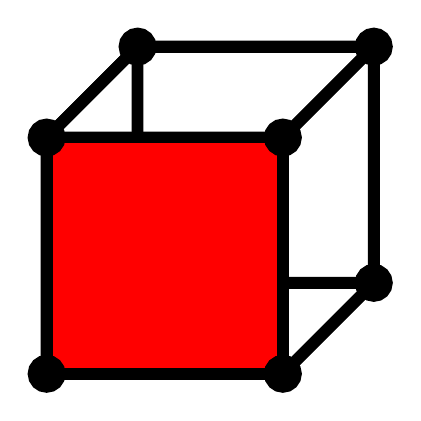
\begin{tikzpicture}[scale=3,line width=1.5mm]

\draw [circle] (1,0,0) -- (1,0,1) -- (1,1,1) -- (1,1,0) -- cycle;
\draw [circle] (0,0,0) -- (0,0,1) -- (0,1,1) -- (0,1,0) -- cycle;

\draw [circle] (0,0,0)   -- (1,0,0)  -- (1,0,1)  -- (0,0,1)  -- cycle;
\draw [circle] (0,1,0)   -- (1,1,0)  -- (1,1,1)  -- (0,1,1)  -- cycle;

\draw [circle] (0,0,0)  node[draw, fill = black] (nodeA) {}  -- (1,0,0)  node[draw, fill = black] (nodeA) {}  -- (1,1,0)  node[draw, fill = black] (nodeA) {}  -- (0,1,0)  node[draw, fill = black] (nodeA) {}  -- cycle;
\draw [circle, fill = red] (0,0,1)  node[draw, fill = black] (nodeA) {}  -- (1,0,1)  node[draw, fill = black] (nodeA) {}  -- (1,1,1)  node[draw, fill = black] (nodeA) {}  -- (0,1,1)  node[draw, fill = black] (nodeA) {}  -- cycle;

\end{tikzpicture} 

	Или конъюнкт $x$, грань $x = 1$
	
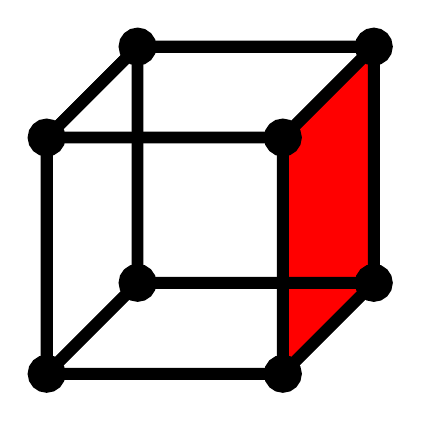
\begin{tikzpicture}[scale=3,line width=1.5mm]

\draw [circle, fill = red] (1,0,0) -- (1,0,1) -- (1,1,1) -- (1,1,0) -- cycle;
\draw [circle] (0,0,0) -- (0,0,1) -- (0,1,1) -- (0,1,0) -- cycle;

\draw [circle] (0,0,0)   -- (1,0,0)  -- (1,0,1)  -- (0,0,1)  -- cycle;
\draw [circle] (0,1,0)   -- (1,1,0)  -- (1,1,1)  -- (0,1,1)  -- cycle;

\draw [circle] (0,0,0)  node[draw, fill = black] (nodeA) {}  -- (1,0,0)  node[draw, fill = black] (nodeA) {}  -- (1,1,0)  node[draw, fill = black] (nodeA) {}  -- (0,1,0)  node[draw, fill = black] (nodeA) {}  -- cycle;
\draw [circle] (0,0,1)  node[draw, fill = black] (nodeA) {}  -- (1,0,1)  node[draw, fill = black] (nodeA) {}  -- (1,1,1)  node[draw, fill = black] (nodeA) {}  -- (0,1,1)  node[draw, fill = black] (nodeA) {}  -- cycle;

\end{tikzpicture} 

\end{example}

	\textbf{Итого:}
	
	$xyz$ ~--- это вершина $x = a, y = b, z = c$

	$xy$ ~--- это ребро $x = a, y = b$ 	

	$x$ ~--- это грань $x = a$ 	

\textbf{Попробуем минимизировать ДНФ}

\begin{example}

	$\overline{x} \: \overline{y} \: \overline{z} \lor x \: \overline{y} \: \overline{z} \lor xy \: \overline{z}$
	
	Найти самый короткий ДНФ для данного выражения
	
	\textbf{Шаг 1: строим ТИ}
	
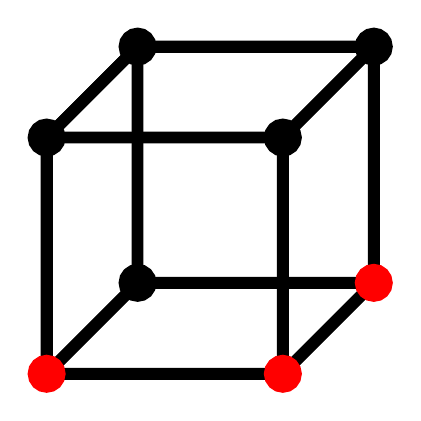
\begin{tikzpicture}[scale=3,line width=1.5mm]

\draw [circle] (1,0,0) -- (1,0,1) -- (1,1,1) -- (1,1,0) -- cycle;
\draw [circle] (0,0,0) -- (0,0,1) -- (0,1,1) -- (0,1,0) -- cycle;

\draw [circle] (0,0,0)   -- (1,0,0)  -- (1,0,1)  -- (0,0,1)  -- cycle;
\draw [circle] (0,1,0)   -- (1,1,0)  -- (1,1,1)  -- (0,1,1)  -- cycle;

\draw [circle] (0,0,0)  node[draw, fill = black] (nodeA) {}  -- (1,0,0)  node[draw, fill = red, red] (nodeA) {}  -- (1,1,0)  node[draw, fill = black] (nodeA) {}  -- (0,1,0)  node[draw, fill = black] (nodeA) {}  -- cycle;
\draw [circle] (0,0,1)  node[draw, fill = red, red] (nodeA) {}  -- (1,0,1)  node[draw, fill = red, red] (nodeA) {}  -- (1,1,1)  node[draw, fill = black] (nodeA) {}  -- (0,1,1)  node[draw, fill = black] (nodeA) {}  -- cycle;

\end{tikzpicture} 

	$\overline{x} \: \overline{y} \: \overline{z} = (0, 0, 0)$
	
	$x \: \overline{y} \: \overline{z} = (1, 0, 0)$
	
	$xy \: \overline{z} = (1, 1, 0)$

	\textbf{Шаг 2: упрощаем}
	
	Чтобы упростить имеет смысл рассмотреть 2 ребра:
	
	$(0, 0, 0) -- (1, 0, 0) = \overline{y} \: \overline{z}$

	$(1, 0, 0) -- (1, 1, 0) = x \: \overline{z}$
	
	$\Rightarrow$ ДНФ $ = \overline{y} \: \overline{z} \lor x \: \overline{z} = \overline{x} \: \overline{y} \: \overline{z} \lor x \: \overline{z} = xy \: \overline{z} \lor \overline{y} \: \overline{z}$
	
	$\Rightarrow$ самое короткое ДНФ $ = \overline{y} \: \overline{z} \lor x \: \overline{z}$

\end{example}

\begin{example}

	$\overline{x} \: \overline{y} \: \overline{z} \lor x \: \overline{y} \lor xy$

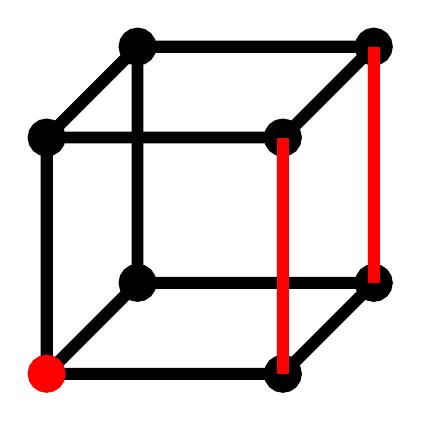
\begin{tikzpicture}[scale=3,line width=1.5mm]

\draw [circle] (1,0,0) -- (1,0,1) -- (1,1,1) -- (1,1,0) -- cycle;
\draw [circle] (0,0,0) -- (0,0,1) -- (0,1,1) -- (0,1,0) -- cycle;

\draw [circle] (0,0,0)   -- (1,0,0)  -- (1,0,1)  -- (0,0,1)  -- cycle;
\draw [circle] (0,1,0)   -- (1,1,0)  -- (1,1,1)  -- (0,1,1)  -- cycle;

\draw [circle] (0,0,0)  node[draw, fill = black] (nodeA) {}  -- (1,0,0)  node[draw, fill = black] (nodeA) {}  -- (1,1,0)  node[draw, fill = black] (nodeA) {}  -- (0,1,0)  node[draw, fill = black] (nodeA) {}  -- cycle;
\draw [circle] (0,0,1)  node[draw, fill = red, red] (nodeA) {}  -- (1,0,1)  node[draw, fill = black] (nodeA) {}  -- (1,1,1)  node[draw, fill = black] (nodeA) {}  -- (0,1,1)  node[draw, fill = black] (nodeA) {}  -- cycle;

\draw [red] (1,1,1) -- (1,0,1);
\draw [red] (1,1,0) -- (1,0,0);

\end{tikzpicture} 

	$\Rightarrow $ ДНФ $ = x \lor \overline{x} \: \overline{y} \: \overline{z} = x \lor \overline{y} \: \overline{z}$

\end{example}

\begin{remark}
	Данный метод позволяет наглядно перебрать все ДНФ и найти минимальный
	
	С помощью алгебраических преобразований мы не сможем понять, что ответ самый оптимальный
\end{remark}

\begin{example}
	Алгебраические преобразования
	
	$\overline{x} \: \overline{y} \: \overline{z} \lor x \: \overline{y} \: \overline{z} \lor xy \: \overline{z} = \overline{x} \: \overline{y} \: \overline{z} \lor x \: \overline{y} \: \overline{z} \lor x \: \overline{y} \: \overline{z} \lor xy \: \overline{z} = \overline{y} \: \overline{z} \lor x \: \overline{z}$
	
	Но тут непонятно, а вдруг можно сделать еще короче
\end{example}

\subsubsection{Двойственная функция}

	Пусть есть логическая функция: $f = B^n \rightarrow B = \{0, 1\}$
	
	Двойственная функция: $f^* = B^n \rightarrow B = \{0, 1\}$
	
	$f^*(x_1, x_2, \dots, x_n) = \overline{f(\overline{x_1}, \overline{x_2}, \dots, \overline{x_n})}$

\begin{remark}
	Мир замены лжи на истину
	
	$$0 \leftrightarrow 1$$
\end{remark}

\begin{example}
	$f(x, y) = x \lor y$
	
	\begin{table}[h!]
		\centering
		\begin{tabular}{|c|c|c|}
			\hline
			$x$ & $y$ & $f$ \\ \hline
			0 & 0 & 0 \\ \hline
			0 & 1 & 1 \\ \hline
			1 & 0 & 1 \\ \hline
			1 & 1 & 1 \\ \hline
		\end{tabular}
	\end{table}
	
	Новый мир: $1 \rightarrow 0, 0 \rightarrow 1$

	\begin{table}[h!]
		\centering
		\begin{tabular}{|c|c|c|}
			\hline
			$x$ & $y$ & $f^*$ \\ \hline
			1 & 1 & 1 \\ \hline
			1 & 0 & 0 \\ \hline
			0 & 1 & 0 \\ \hline
			0 & 0 & 0 \\ \hline
		\end{tabular}
	\end{table}
	
	Получилось, что $(x \lor y)^* = xy$
\end{example}

\begin{example}
	$(x \lor y)^* = \overline{\overline{x} \lor \overline{y}} = \overline{\overline{x}} \: \overline{\overline{y}} = xy$
\end{example}

\begin{example}
	$(x + y)^* = \overline{\overline{x} + \overline{y}} = \overline{1 + x + 1 + y} = 1 + x + 1 + y + 1 = 1 + x + y = x \Leftrightarrow y$
\end{example}

\begin{remark}
	$f^{**}(x_1, x_2 \dots x_n) = \overline{f^*(\overline{x_1}, \overline{x_2} \dots \overline{x_n})} = \overline{\overline{f(x_1, x_2 \dots x_n)}} = f(x_1, x_2 \dots x_n)$
\end{remark}

\begin{corollary}
	$$(xy)^* = x \lor y$$
	
	$$(x \Leftrightarrow y)^* = x + y$$
\end{corollary}

	\textbf{Теорема о композиции:}
	
	$f = f_0(f_1(x_1, \dots x_n), f_2(x_1, \dots x_n), \dots f_m(x_1, \dots x_n))$
	
	$f_i$ ~--- это функции от n переменных $(B^n \rightarrow B) (i = 1 \dots n)$
	
	$f_0 = B^m \rightarrow B$
	
	Тогда $f^*(x_1, \dots x_n) = f^{*}_{0}(f^{*}_{1}(x_1, \dots x_n), f^{*}_{2}(x_1, \dots x_n), \dots f^{*}_{m}(x_1, \dots x_n))$
	
	\textbf{Доказательство:}
	
	$f^* = \overline{f(\overline{x_1}, \dots \overline{x_n})} =  \overline{f_0(f_1(\overline{x_1}, \dots \overline{x_n}), f_2(\overline{x_1, \dots \overline{x_n}}) \dots f_m(\overline{x_1}, \dots \overline{x_n}))} = f_0^*(\overline{f_1(\overline{x_1, \dots \overline{x_n}}), \overline{f_2(\overline{x_1}, \dots \overline{x_n})}, \dots \overline{f_m(\overline{x_1}, \dots \overline{x_n})}}) $

\begin{corollary}
	Если есть $f(x_1, \dots x_n)$ ~--- записано, как логическое выражение с $\cdot, \: \lor, \: \neg, \: +, \: \Leftrightarrow$, то $f^*$ ~--- также выражение, но связки заменяются на двойственные узлы
	
	$$\lor \leftrightarrow *$$

	$$+ \leftrightarrow \Leftrightarrow$$
	
	$$\neg \leftrightarrow \neg$$
	
	так как $(\overline{x})^* = \overline{x}$
\end{corollary}

\begin{example}

	$$f(x, y, z) = \overline{x \lor \overline{y} \: z} \Leftrightarrow (x + y + z)$$
	
	$$f^*(x, y, z) = (\overline{x \cdot (\overline{y} \: z)}) + (x \Leftrightarrow y \Leftrightarrow z)$$
\end{example}

\begin{example}

	$$f(x_1, \dots x_n) = 1$$
	
	$$\Rightarrow f^*(x_1, \dots x_n) = \overline{1} = 0$$
	
	$$1^* = 0; 0^* = 1$$
\end{example}

\subsubsection{Конъюнктивно-нормальная форма КНФ}

\begin{definition}
	Конъюнктивно-нормальная форма ~--- еще одна нормальная форма, похожая на ДНФ
\end{definition}

\begin{definition}
	Литерал ~--- это как и раньше, переменные или отрицательные переменные
	
	$$x, y, \overline{x}, \: \overline{y}$$
\end{definition}

\begin{definition}
	Дизъюнкт ~--- дизъюнкция литералов
	
	$$x \lor y; \: x \lor y \lor \overline{z}; \: x \lor \overline{z}; \: \overline{x}$$
	
	$$\cancel{xy}, \cancel{x \lor yz}$$
\end{definition}

\begin{definition}
	КНФ ~--- это конъюнкция нескольких дизъюнктов
	
	$$(x \lor y)(y \lor \overline{z});$$
	
	$$(x \lor \overline{y} \lor z)(\overline{y} \lor \overline{z})(\overline{x})$$
	
	$$\cancel{xy \lor z}$$
	
	$$x \lor y \lor z$$ ~--- 1 дизъюнкт
	
	$$xyz$$ ~--- 3 дизъюнкта
\end{definition}

\end{sloppypar}

	\begin{definition}
		У любой логической функции есть КНФ, её можно построить по таблице истинности
		\end{definition}

	\textbf{Доказательство}

		Заметим,что если вычислить (КНФ$)^{*}$ (двойственную к КНФ), то получим ДНФ

	\begin{example}
	$[(x \vee y \vee z)(x \vee \bar{y})(\bar{y} \vee \bar{z})]^{*} = (xyz)\vee(x\bar{y})\vee(\bar{y}\bar{z})$

		И наоборот (ДНФ$)^{*} = $ КНФ
		\end{example}

	Итого, чтобы получить КНФ для функции f, надо построить двойственную функцию
	к ДНФ это функции. Отсюда следует, что КНФ всегда существует

	\begin{example}
		f(x,y,z) = xy $\Leftrightarrow$ z

		\begin{table}[h!]
	\centering
	\begin{tabular}{|c|c|c|c|c|c|}
		\hline
		$x$ & $y$ & $z$ & $xy$ & $f$ & $f^{*}$ \\ \hline
		0 & 0 & 0 & 0   & 1   & 0   \\ \hline
		0 & 0 & 1 & 0   & 0   & 1   \\ \hline
		0 & 1 & 0 & 0   & 1   & 1   \\ \hline
		0 & 1 & 1 & 0   & 0   & 0   \\ \hline
		1 & 0 & 0 & 0   & 1   & 1   \\ \hline
		1 & 0 & 1 & 0   & 0   & 0   \\ \hline
		1 & 1 & 0 & 1   & 0   & 1   \\ \hline
		1 & 1 & 1 & 1   & 1   & 0   \\ \hline
	\end{tabular}

\end{table}


			Выпишем значения xyz из строчек, где $f^{*} = 1$

			$\bar{x}\bar{y}z$ \quad $x\bar{y}\bar{z}$ \quad $\bar{x}y\bar{z}$ \quad $xy\bar{z}$


		\end{example}

	Вспомним определение $f^{*}(x,y,z) = \overline{f(\bar{x},\bar{y},\bar{z})}$

	$f^{*}(0,0,0) = \overline{f(1,1,1)}$

	Итого: $f^{*}$ = $\bar{x}\bar{y}z \vee \bar{x}y\bar{z} \vee x\bar{y}\bar{z} \vee xy\bar{z}$

	$f^{*}(0,0,1) = \overline{f(1,1,0)}$

	$f^{*}(0,1,0) = \overline{f(1,0,1)}$

	По теореме о композиции

	$f = (\bar{x} \vee \bar{y} \vee z)(\bar{x} \vee y \vee \bar{z})(x \vee \bar{y} \vee \bar{z})(x \vee y \vee \bar{z})$

	Получение КНФ по таблице истинности без двойственной функции

f(x,y,z) = xy $\Leftrightarrow$ z

	\begin{table}[h!]
	\centering
	\begin{tabular}{|c|c|c|c|}
		\hline
		$x$ & $y$ & $z$ & $f = xy \Leftrightarrow z $\\ \hline
		0 & 0 & 0 	& 1  \\ \hline
		0 & 0 & 1 	& 0  \\ \hline
		0 & 1 & 0 	& 1  \\ \hline
		0 & 1 & 1 	& 0  \\ \hline
		1 & 0 & 0 	& 1  \\ \hline
		1 & 0 & 1 	& 0  \\ \hline
		1 & 1 & 0 	& 0  \\ \hline
		1 & 1 & 1 	& 1  \\ \hline
	\end{tabular}
\end{table}


		При x y z = 1 1 0, f= xy $\Leftrightarrow$ z $\leftarrow$ $\bar{x}\lor\bar{y}\lor z$

	для 1 - отрицание, для 0 - нет отрицания

	Итого: Чтобы построить ДНФ:

	- строки с 1, $0 \leftrightarrow \bar{x}\bar{y}\bar{z}$

	\qquad \qquad \qquad $1 \leftrightarrow xyz$

	Чтобы получить КНФ:

	- строки с 0, 0 $\leftrightarrow xyz$

	\qquad \qquad \qquad 1 $\leftrightarrow \bar{x}\bar{y}\bar{z}$

	\begin{example}
	f = x+y

	\begin{table}[h!]
	\centering
	\begin{tabular}{|c|c|c|}
		\hline
		$x$ & $y$ & $x+y$ \\ \hline
		0 & 0 & 0 \\ \hline
		0 & 0 & 1 \\ \hline
		0 & 1 & 1 \\ \hline
		0 & 1 & 0 \\ \hline
	\end{tabular}
\end{table}


	Нули в: $x \lor y \qquad \bar{x} \lor \bar{y}$

	$f = (x\lor y)(\bar{x} \lor \bar{y})$



\end{example}

	\begin{remark}
		Для функции записанной в форме КНФ, можно поставить задачу "выполнимости".

		Вопрос: может ли значение быть = 1

		- не известно решений, принципиально эффективней полного перебора значений

		\end{remark}

	\begin{example}
	$(x \lor y \lor z)(x \lor \bar{y})(y \lor \bar{z})(\bar{x} \lor \bar{z}) = 1$

		x = 1

		y = 1 \qquad подходит

		z = 0

		Cледовательно эта формула выполнима при таком наборе


	\end{example}

	Многие задачи, головоломки сводятся к задаче выполнимости

	\begin{example}
		Прицнцип Дирихле

			Если есть n клеток и в них n+1 заяц, то $\exists$ клетка, где зайцев $\geqslant$ 2.

		при n = 2: i = 1 или 2 (клетка) \qquad $x_{ij} $ - в клетке i сидит заяц j

		\qquad \qquad \quad j = 1 или 2 или 3 заяц

		Попробуем записать, что в каждой клетке $\leqslant$ 1 зайца

		а) каждый заяц ровно в одной клетке

		$x_{11} \oplus x_{21}$ - заяц 1

		$x_{12} \oplus x_{22}$ - заяц 2

		$x_{13} \oplus x_{23}$ - заяц 3

		б) в каждой клетке не больше 1 зайца

			\begin{table}[h!]
	\centering
	\begin{tabular}{|c|c|c|c|}
		\hline
		кл/з & $1$ & $2$ & $3$ \\ \hline
		1 & $x_{11}$ & $x_{12}$ & $x_{13}$ \\ \hline
		2 & $x_{21}$ & $x_{22}$ & $x_{23}$ \\ \hline
	\end{tabular}
\end{table}

		если есть 2 зайца, то один из конъюнктов: = 1

		$\overline{x_{11}x_{12} \lor x_{11}x_{13} \lor x_{12}x_{13}} \longleftarrow$ в кл $1 \leqslant 1$ зайца

		$\overline{x_{21}x_{22} \lor x_{21}x_{23} \lor x_{22}x_{23}} \longleftarrow$ в кл $2 \leqslant 1$ зайца

		Соединяем все утверждения:
		
	$(x_{11} + x_{21})(x_{12} + x_{22})(x_{13} + x_{23})(\overline{x_{11}x_{12} \lor x_{11}x_{13} \lor x_{12}x_{13}})(\overline{x_{21}x_{22} \lor x_{21}x_{23} \lor x_{22}x_{23}}) = 0$ всегда из принципа Дерихле
	 
	 $(x_{11} \lor x_{21})(\overline{x_{11}} \lor \overline{x_{21}})(x_{12} \lor x_{22})(\overline{x_{12}} \lor \overline{x_{22}})(x_{13} \lor x_{23})(\overline{x_{13}} \lor \overline{x_{23}})(\overline{x_{11}} \lor \overline{x_{12}})(\overline{x_{11}} \lor \overline{x_{13}})(x_{12} \lor x_{13})(\overline{x_{21}} \lor \overline{x_{22}})(\overline{x_{21}} \lor \overline{x_{23}})(\overline{x_{22}} \lor \overline{x_{23}})$
	
		$\longleftarrow$
		Берем программу, которая решает КНФ задачу выполнимости. Она скажет - невозможно.

		\end{example}

	\subsubsection{Класс замкнутости}

	Повторим: Логическая функция: f: $\beta^{n} \rightarrow \beta$

	$\beta = \{0,1\}$

	\begin{definition}
		Класс ~-- это множество логических функций.
	\end{definition}

	\begin{example}

		$K_{1} = $ класс функций: от двух переменных
		$K_{2} = $ класс функций такой, что $f(x,y) = f(y,x)$

		$f(x,y) = x \lor y \in K_{1}, \in K_{2}$

		$g(x,y) = x \Rightarrow y \in K_{1} \notin K_{2}$

		$K_{3}:$ класс функций $f(x,...) = f(\overline{x}, ...)$
		функции, которые не зависят от первой переменной

		$f(x,y,z) = y \Rightarrow z \in K_{3}$

		$f(x,y,z) = (x \Rightarrow y) \lor z \notin K_{3}$

		$f(x,y,z) = x\bar{x} \lor y \lor z \in K_{3}$ \quad $(x \bar{x})$

		$K_{4}: \{f(x,y) = x \lor y;$  $ g(x,y) = x \Rightarrow y\}$

		\end{example}

		\begin{definition}
			Замыкание класса

			$K = \{f_{1},f_{2},\dots\}$ ~--- класс функции

			\end{definition}
			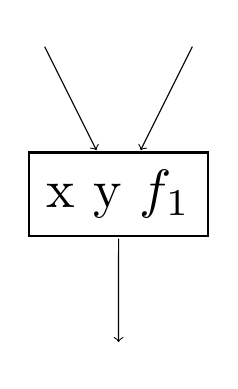
\begin{tikzpicture}
		\node (first_diag)[scale = 1.5, style = {thick, draw = black}]
		[scale = 1.3] at ( 0,0) {x y $f_{1}$};
		\node (1) at ( 1,2) {};
		\node (2) at ( -1,2) {};
		\node (3) at ( 0,-2) {};
		\path(1) edge[->] (first_diag);
		\path(2) edge[->] (first_diag);
		\path(first_diag) edge[->] (3);
	\end{tikzpicture}
			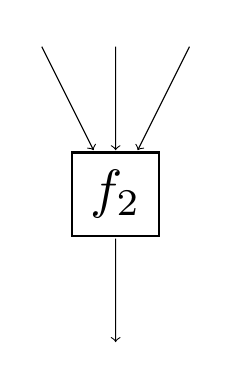
\begin{tikzpicture}
		\node (first_diag)[scale = 1.5, style = {thick, draw = black}]
		[scale = 1.3] at ( 1,1) {$f_{2}$};
		\node (1) at ( 0,3) {};
		\node (2) at ( 2,3) {};
		\node (3) at ( 1,3) {};
		\node (4) at ( 1,-1) {};
		\path(1) edge[->] (first_diag);
		\path(2) edge[->] (first_diag);
		\path(3) edge[->] (first_diag);
		\path(first_diag) edge[->] (4);
	\end{tikzpicture}

			$K^{*}$ ~--- замыкание класса - это класс состоящий из всех композиций функций из K


			\frame{$f_{1}(f_{2})(f_{1}(x,y),y,z),z)$} ~--- композиция

			если есть функции, подставляем друг в друга, получаем композицию

	\begin{example}
		$:1) K = \{0,\bar{x}\}$ \quad (0 - f() $\bar{x} - g(x)$)

		$K^{*} = \{ f(), g(f()), g(g(f())), g(g(g(f())))\}$
\end{example}
	\begin{example}
		$K = \{\bar{x}\}$ возьмем класс только из отрицательных

		$K^{*} = \{ \bar{x}, x\}$

		$K = \{ g(x), g((g(x))), g(g(g(x \dots 1, \dots )))\}$
\end{example}
	\begin{example}
		$K^{*}=\{ \bar{x}$,$ x \lor y$,$ xy \}$  $\quad K^{*} = \{ $,$ \dots$,$ \forall$, функция $\}$
	\end{example}

	\begin{definition}

		Если К - класс:

		$K^{*} = \alpha$, то \frame{К - полный}, где $\alpha$ ~--- все логические функции

		Вывод: $K = \{ \bar{x}, x \lor y, xy\}$ ~--- полный

		\end{definition}
		\begin{example}

			$K = \{\bar{x}, x \lor y \}$, где $f(x) = \bar{x}$, $g(x, y) = x \lor y$
		\end{example}
		
		$xy = \overline{\overline{xy}} = \overline{\overline{x} \lor \overline{y}}
		 = f(g(f(x),f(y)))$  % need check

		Значит $K^{*}$ ~--- тоже полный


	\begin{definition}
		Замкнутый класс ~~- K замкнут, если $K^{*} = K$
		\end{definition}

	Свойства замыкания:

	1. $K_{1} \subset K_{2}$, тогда $K_{1}^{*} \subset K_{2}^{*}$

	\textbf{Докозательство:}

		Если есть f $\in K_{1}^{*} \Rightarrow f = $ композиция $f_{1} \in K_{1} \Rightarrow$
	f - композиция $(f_{i} \in K_{2}) \Rightarrow f \in K_{2}^{*} $ чтд.

	2.Если $K_{1} \subset K_{2}$ и $K_{1}$ - полный, то $K_{2}$ - полный

	\textbf{Докозательство:}

	$K_{1} \subset K_{2} \Rightarrow K_{1}^{*} \subset K_{2}^{*} \Rightarrow \alpha
	 \subset K_{2}^{*} \Rightarrow K_{2}^{*} = \alpha
	$

	3. Пусть $K_{1}$, $K_{2}$ ~~- замкнутое, тогда $K_{1} \cap K_{2}$ ~~- тоже замкнутые

	\textbf{Докозательство:}

	Пусть есть $f = (K_{1} \cap K_{2})^{*} $ ~~- композиция

	$f_i \in (K_{1} \cap K_{2})$

	а) $\Rightarrow f_i $ ~~- композиция $ f_i = K_1 \Rightarrow f \in K_{1}^{*}$

	б) $\Rightarrow f_i $ - композиция $f_i = K_2 \Rightarrow f \in K_{2}^{*}$

	Из а и б следует, что $ f \in K_{1}^{*} \cap K_{2}^{*} = K_{1} \cap K_{2}$

	Итог: $f \in (K_{1} \cap K_{2})^{*} \Rightarrow f \in K_{1} \cap K_{2}$ 

	$\Rightarrow	(K_{1} \cap K_{2})^{*} \subset K_{1} \cap K_{2}$, 
	по $K_{1} \cap K_{2} \subset (K_{1}
	\cap K_{2})^{*}$ 
	
	$\Rightarrow K_{1} \cap K_{2} = (K_{1} \cap K_{2})^{*}$
	
	$\Rightarrow K_{1} \cap K_{2} $ - замкнут

	\begin{remark}
		$K_{1}$ и $K_{2}$ - замкнутые $\Rightarrow K_{1} \cup K_{2} $ - замкнутый
		\end{remark}

	4. $K^{*} = K^{**}$ для любого класса функций

	\subsubsection{Примеры замкнутых классов}

	1. $T_{0}$ - класс функций, "сохраняющих ноль" $f \in T_{0} \Leftrightarrow$  если
	$f(0,....0) = 0$

	$x*y \in T_{0}$

	$x+y \in T_{0}$

	$\bar{x} \notin T_{0}$

	$x \Rightarrow y \notin T_{0}$

	$xy + xz + yz \in T_{0}$

	\textbf{Утверждение:} $T_{0} $ - замкнут

	\textbf{Докозательство:}

	$\sqsupset f \in T_{0}^{*}$, проверим, что $f \in T_{0}$

	$\Rightarrow T_{0}^{*} \subset T_{0}$

	$\Rightarrow T_{0}^{*} = T$

	f - комп $f_{i}$, $f_{i} \in T_{0}$

	$f_{1}(f_{2}(...)f_{3}(f_{4}(...)),...)$ - композиция

	подставим все 0

	$\Rightarrow f(0,....0) = 0 \Rightarrow f \in T_{0} $ чтд

	\begin{example}
		$f_{1}(x,y) = x*y$ \qquad $f_{1} \in T_{0} f_{2} \in T_{0}$

		$f_{2}(x,y) = x+y$ \qquad $f_{1}(f_{2}(f_{1}(x,f_{2}(y,y)),y)f_{1}(z,z))$

		$x(y+y)$

		$f(x,y,z) = (x(y+y)+y)*z*z$

		$f(0,0,0) = 0$

		2. Класс $T_{1}$ - сохраняющие 1

		$f \in T_{1}$, если $f(1,...1) = 1$

		$x*y \in T_{1}$

		$x+y \notin T_{1}$

		$x+y+z \in T_{1}$

		$\bar{x} \notin T_{1}$

		$x \Rightarrow y \in T_{1}$

		$xy + xz + yz \in T_{1}$

		\begin{proposition}
			$T_{1}$ - замкнут
			\end {proposition}


		\textbf{Докозательство:} смотри $T_{0}$

		3. Класс $\frame{\&}$

		$f \in \frame{\&}$, если f можно записать как конъюнкцию нескольких переменных

		$f(x,y,z) = yz$

		$g(x,y,z) = xyz$

		$h(x,y,z) = xz$

		$i(x,y,z) = z$

		0

		1

		Все это $\in \frame{\&}$

		\begin{proposition}
			Класс $\frame{\&}$ замкнут
			\end{proposition}

		Композиция $f_{i} \in \frame{\&}$

		$f_1(...,\frame{...},...,\frame{...}) = $ арг2 * арг4 = подаргумент1* подаргумент2* ... * подаргумент =
		пер * пер * пер * пер... (произвольная переременная)

		пер может быть 0 или 1

		\begin{proposition}
			$\frame{\&} = \{\&,0,1\}^{*}$

			по определению замыкания

			$\{f_{1}(x,y) = x*y$

			$f_{2}() = 0$

			$f_{3}() = 1\}$

			\end{proposition}

		4. \frame{V} - дизъюнкция переменных и 0, 1

		\frame{V} = $\{V,0,1\}^{*}$

		\begin{proposition}

			$\frame{V} $ - замкнут

			\end{proposition}

		\textbf{Докозательство 1: }

		смотри докозательство $\frame{\&}$


		\textbf{Докозательство 2: }

		$\frame{V} = \{V,0,1\}^{*}$ 
		$\Rightarrow \frame{V}^{*} = \{V,0,1\}^{**} = \{V,0,1\}^{*} = \frame{V}$ свойства замыкания

		\end{example}

	\textbf{Докозательство: } $\sqsupset  f \in K^{*} \Rightarrow f - $ комп $f_{i}
	\Rightarrow f_{i} \in K^{*}
	$

	$ f = f_{1} (f_2(...)...) = g_{1}(g_{2}(h_{1}...)) \in k^{*}
	$

	\qquad $\uparrow$ \quad $\uparrow$ \qquad комп $g_{1} \in K^{*}$

	$g_{i} \in K $ $h_{i} \in K$

	$\Rightarrow f \in K^{*} \Rightarrow K^{*} = K^{**}$

	Следствие: $\forall K$ - класс $K^{*}$ - замкнут

	если класс замкнут он станет замкнутым

	5. Класс u (unit) : 0,1,$f(x,...x_{n}) = x_{i}$ или  $\overline{x_{i}}$

	$f(x,y,z) = \bar{z}$

	$f(x,y,z,t) = x$

	$f(x) = x f(x) = \bar{x}$

	Все это $\in u$

	6. Класс $1^{\infty}$ $f(x_{1}...x_{n}) \leqslant x_{i} $

	\qquad $0^{\infty} f(x...x_{n}) \geqslant x_{i}$

	$x*y \leqslant x$ \qquad $xy \in 1^{\infty}$

	\quad $\leqslant y$

	$x \lor y \geqslant x$ \qquad $x \lor y \in 0^{\infty}$

	\quad $\geqslant y$

	$x \Rightarrow y \geqslant y$ \quad $x \Rightarrow y \in 0^{\infty} $

	$x \Rightarrow y \leqslant y $

	\qquad $x=0$

	\qquad $y=0$

	$x \Rightarrow y \notin 1^{\infty}$

	7. L - линейная функция L = $\{0,1,+\}^{*}$

	Все функции из констант и сложения

	$x+y \in L$

	$x+y + z \in L$

	$1+x \in L$

	$\bar{x} \in$

	$x * y \in L$

	(L - линейные многочлены Жегалкина, степени $\leqslant$ 1)

	\textbf{Докозательство: } $ x * y$ имеет многочлены Жегалкина $x*y$

	он единственный $\Rightarrow $ не существует линейного многочлена Жегалкина %do

	8. S - самодвойствейнные функции

	$f \in S$, если f = $f^{*}$ \quad ($f^{*} $ - двойственные)

	Если функция равна своей двойственной, то она самодвойтсвенная

	\begin{example}
		$x*y \notin S$

		$x \lor y \notin S$

		$x \in S$

		$\bar{x} \in S$

		$x \Rightarrow y \notin S $ т.к. $(x \Rightarrow y)^{*} = (\bar{x} \lor y)^{*} = \bar{x}*y \neq \bar{x} \lor y$

		$x = 1$
		\end{example}
	Функция честного голосования $y = 1$ от 3 ёх переменных. $0 \neq 1$

	$vote(x,y,z) = 1$,  если 1 - иц больше $x + y + z \geq z$

	 \qquad \quad \quad \quad \quad \quad 0, если 0 - ей больше $x + y + z \leq 1$

	$vote(x,y,z)$ : Таблица истинности


	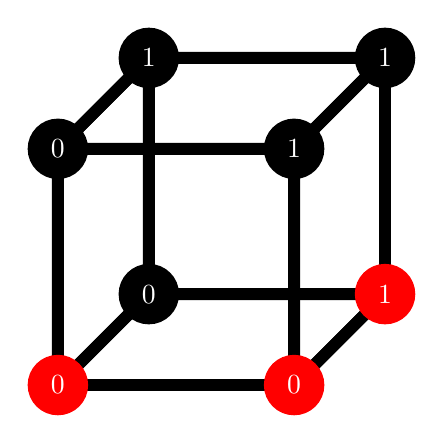
\begin{tikzpicture}[scale=3,line width=1.5mm]

\draw [circle] (1,0,0) -- (1,0,1) -- (1,1,1) -- (1,1,0) -- cycle;
\draw [circle] (0,0,0) -- (0,0,1) -- (0,1,1) -- (0,1,0) -- cycle;

\draw [circle] (0,0,0)   -- (1,0,0)  -- (1,0,1)  -- (0,0,1)  -- cycle;
\draw [circle] (0,1,0)   -- (1,1,0)  -- (1,1,1)  -- (0,1,1)  -- cycle;

\draw [circle] (0,0,0)  node[draw, fill = black] (nodeA) {\textcolor{white}{0}}  -- (1,0,0)  node[draw, fill = red, red] (nodeA) {\textcolor{white}{1}}  -- (1,1,0)  node[draw, fill = black] (nodeA) {\textcolor{white}{1}}  -- (0,1,0)  node[draw, fill = black] (nodeA) {\textcolor{white}{1}}  -- cycle;
\draw [circle] (0,0,1)  node[draw, fill = red, red] (nodeA) {\textcolor{white}{0}}  -- (1,0,1)  node[draw, fill = red, red] (nodeA) {\textcolor{white}{0}}  -- (1,1,1)  node[draw, fill = black] (nodeA) {\textcolor{white}{1}}  -- (0,1,1)  node[draw, fill = black] (nodeA) {\textcolor{white}{0}}  -- cycle;

\end{tikzpicture}

	$vote(x,y,z) \in S$?

	$(xy \lor xz \lor yz)^{*} = (x \lor y)(x \lor z)(y \lor z) =? xy \lor xz \lor yz$

	Раскроем скобки:

	$xxy \lor xxz \lor xzy \lor xzz \lor yxy \lor yxz \lor yzy \lor yzz =
	xy \lor xz \lor xyz \lor xz \lor xy \lor xyz \lor yz \lor yz = xy \lor
	xz \lor yz \lor xyz = xy \lor xz \lor yz(1 \lor x) = xy \lor xz \lor yz$

	т.е. vote = $vote^{*}$

	или проверим таблицой истинности:

	читаем снизу вверх, заменяя 0 на 1

	\begin{table}[h!]
	\begin{tabular}{|c|c|c|}
		\hline
		$xyz$ & $vote$ & $vote^{*}$ \\ \hline
		000 & 0 & 0 \\ \hline
		001 & 0 & 0 \\ \hline
		010 & 0 & 0 \\ \hline
		011 & 1 & 1 \\ \hline
		100 & 0 & 0 \\ \hline
		101 & 1 & 1 \\ \hline
		110 & 1 & 1 \\ \hline
		111 & 1 & 1 \\ \hline
\end{tabular}
\end{table}

	\begin{proposition}

		S - замкнут

		$\sqsupset f \in S^{*} f = $композиция $f_{i} \in S$

		$f = f_{i}(f_{2}(...),f_{3}(...),f_{4}(...))$

		\end{proposition}

	\begin{definition}

		Высота композиции

		$f(x,y,z)$ - высота 1 (1 ф-ия)

		$f(g(x,y),y,z)$ - высота 2

		$g(x,y) - 1$

		$f(g(x,y),y,z) - 2$
		\end{definition}


	\begin{example}
	$f(g(h(x),y),h((h(x)),y))$

	$g(h(x),y)$ - 2

	$h(h(x))$ - 2

	$f(g(h(x),y),h((h(x)),y))$ - 3

	\end{example}

	$f^{*} = f_{1}^{*}(f_{2}^{*}(...),  ,f_{n}^{*}(...))$ - теория о композиции

	но $f_{i} \in S \Rightarrow f_{i}^{*} = f_{i}$

	$= f_{i}(f_{2}(...),...f_{n}(...)) = f$

	т.е $f^{*} = f \Rightarrow f \in S$
	
	9. Монотонные функции
	
	$f(x_1, \dots, x_n) \in M$, если $\forall i \quad x_i \geq y_i$
	
	$\Rightarrow f(x_1, \dots, x_n) \geq f(y_1, \dots, y_n)$

\end{document}